\documentclass[11pt]{article}
\usepackage{geometry}
\usepackage{graphicx}
\usepackage{amsmath}
\usepackage[twoside]{fancyhdr}
\usepackage{lastpage}
\pagestyle{fancyplain}
\setlength{\headheight}{13.6pt}
\fancyhf{}
\lhead{ \fancyplain{}{CS271: Data Structures} }
\rhead{ \fancyplain{}{Fall 2025} }
\fancyfoot[RO, LE] {page \thepage\ of \pageref{LastPage} }
\thispagestyle{plain}

\usepackage{amsthm}
\newtheorem{theorem}{Theorem}
\newtheorem{lemma}{Lemma}

\usepackage{tikz}
\usetikzlibrary{arrows,positioning, calc}
\tikzstyle{inheap}=[draw,circle,minimum size=20pt,inner sep=0pt]
\tikzstyle{outheap}=[draw,fill=black!15,circle,minimum size=20pt,inner sep=0pt]

\begin{document}
\begin{center}
{\Large \textsc{CS271: Data Structures}}\vspace{\baselineskip}\\

Name: YOUR NAMES HERE\vspace{\baselineskip}\\
Instructor: Dr. Stacey Truex
\vspace{\baselineskip}\\
\Large{Unit 1: Practice 1}
\end{center}

\section*{Time Breakdown}

Each group member certifies that 1 hour (60 minutes) -- please note that \textbf{no more than 1 hour} is required -- was spent \textit{collaboratively} on Unit 1 Practice 1 material. The breakdown of how those 60 minutes were spent is as follows:
\begin{itemize}
    \item 
\end{itemize}

\section*{Practice}

\begin{enumerate}

    \item\label{tree} Draw the following array as a nearly complete binary tree:
    \[[7,50,3,46,51,42,36,45,69,94]\]

    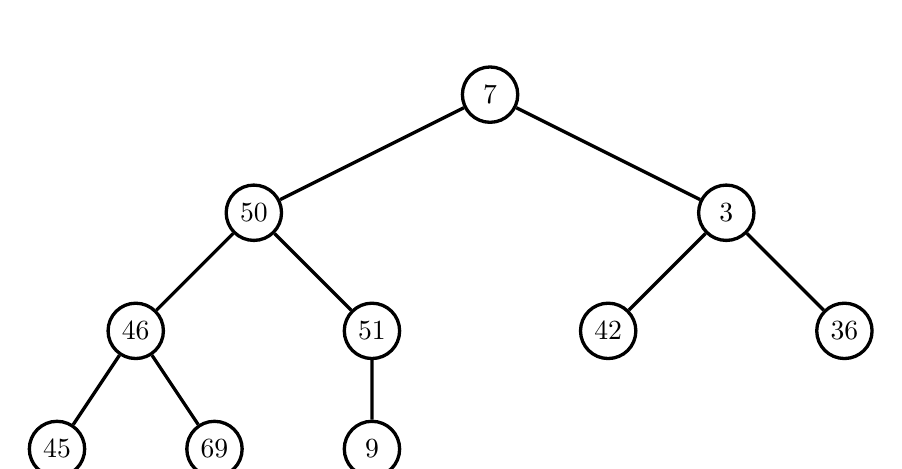
\begin{tikzpicture}[very thick,level/.style={sibling distance=60mm/#1}]
    \node [inheap] {7}
      child {
        node [inheap] {50}
        child {
          node [inheap] {46}
          child {
            node [inheap] {45}}
          child {node [inheap] {69}}
        }
        child {
          node [inheap] {51}
          child {node [inheap] {9}}
        }
      }
      child {
        node [inheap] {3}
        child {
          node [inheap] {42}}
        child {
          node [inheap] {36}}
      };
    \end{tikzpicture}

    \item\label{heap} Fill in the following images corresponding to the state of the binary tree from (\ref{tree}) at the end of each iteration of the \texttt{for} loop in the \textsc{Build-Max-Heap} algorithm. List which values were swapped in the call to \textsc{Max-Heapify}.

    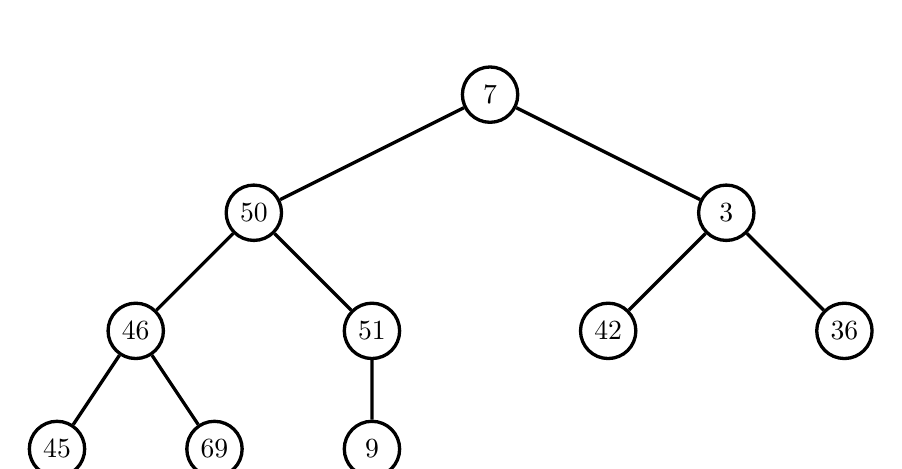
\begin{tikzpicture}[very thick,level/.style={sibling distance=60mm/#1}]
    \node [inheap] {7}
      child {
        node [inheap] {50}
        child {
          node [inheap] {46}
          child {
            node [inheap] {45}}
          child {node [inheap] {69}}
        }
        child {
          node [inheap] {51}
          child {node [inheap] {9}}
        }
      }
      child {
        node [inheap] {3}
        child {
          node [inheap] {42}}
        child {
          node [inheap] {36}}
      };
    \end{tikzpicture}

    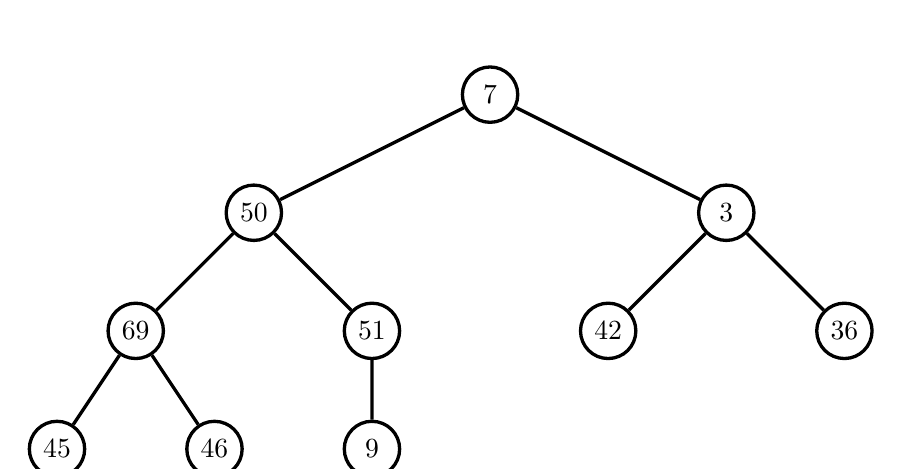
\begin{tikzpicture}[very thick,level/.style={sibling distance=60mm/#1}]
    \node [inheap] {7}
      child {
        node [inheap] {50}
        child {
          node [inheap] {69}
          child {
            node [inheap] {45}}
          child {node [inheap] {46}}
        }
        child {
          node [inheap] {51}
          child {node [inheap] {9}}
        }
      }
      child {
        node [inheap] {3}
        child {
          node [inheap] {42}}
        child {
          node [inheap] {36}}
      };
    \end{tikzpicture}

    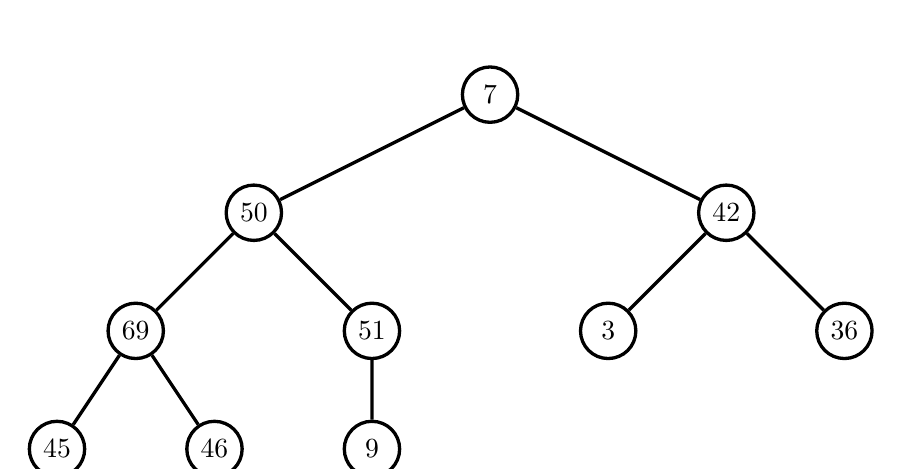
\begin{tikzpicture}[very thick,level/.style={sibling distance=60mm/#1}]
    \node [inheap] {7}
      child {
        node [inheap] {50}
        child {
          node [inheap] {69}
          child {
            node [inheap] {45}}
          child {node [inheap] {46}}
        }
        child {
          node [inheap] {51}
          child {node [inheap] {9}}
        }
      }
      child {
        node [inheap] {42}
        child {
          node [inheap] {3}}
        child {
          node [inheap] {36}}
      };
    \end{tikzpicture}

    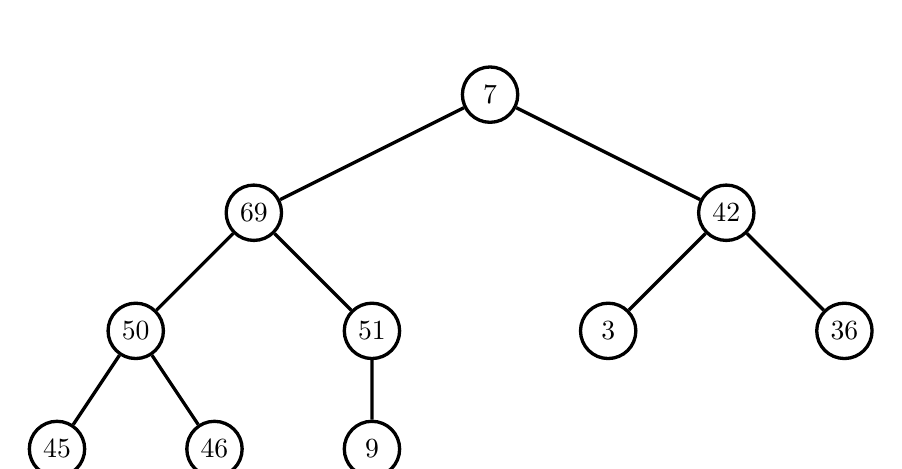
\begin{tikzpicture}[very thick,level/.style={sibling distance=60mm/#1}]
    \node [inheap] {7}
      child {
        node [inheap] {69}
        child {
          node [inheap] {50}
          child {
            node [inheap] {45}}
          child {node [inheap] {46}}
        }
        child {
          node [inheap] {51}
          child {node [inheap] {9}}
        }
      }
      child {
        node [inheap] {42}
        child {
          node [inheap] {3}}
        child {
          node [inheap] {36}}
      };
    \end{tikzpicture}

    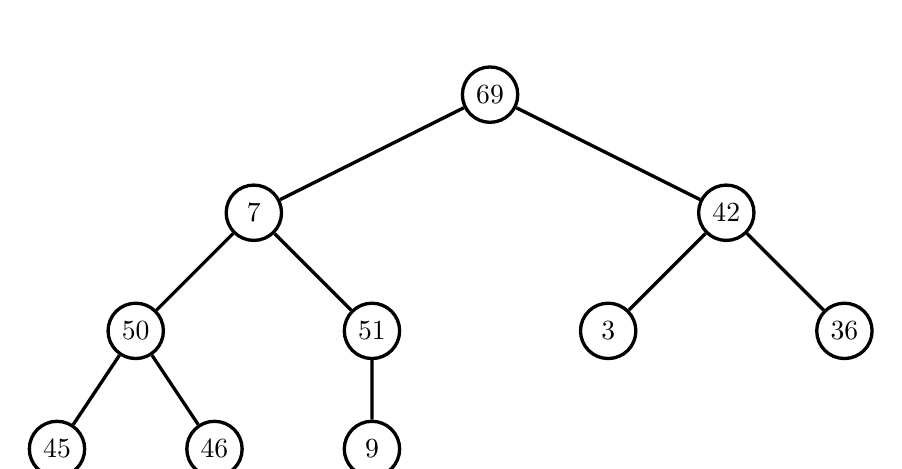
\begin{tikzpicture}[very thick,level/.style={sibling distance=60mm/#1}]
    \node [inheap] {69}
      child {
        node [inheap] {7}
        child {
          node [inheap] {50}
          child {
            node [inheap] {45}}
          child {node [inheap] {46}}
        }
        child {
          node [inheap] {51}
          child {node [inheap] {9}}
        }
      }
      child {
        node [inheap] {42}
        child {
          node [inheap] {3}}
        child {
          node [inheap] {36}}
      };
    \end{tikzpicture}

    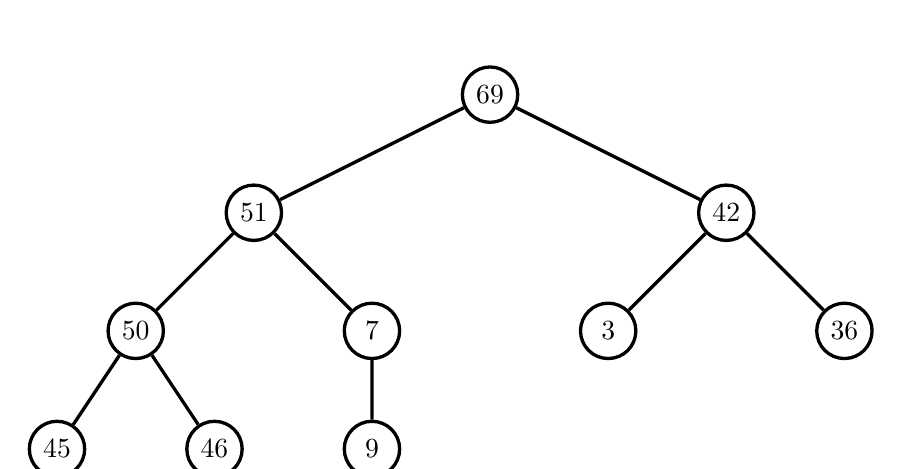
\begin{tikzpicture}[very thick,level/.style={sibling distance=60mm/#1}]
    \node [inheap] {69}
      child {
        node [inheap] {51}
        child {
          node [inheap] {50}
          child {
            node [inheap] {45}}
          child {node [inheap] {46}}
        }
        child {
          node [inheap] {7}
          child {node [inheap] {9}}
        }
      }
      child {
        node [inheap] {42}
        child {
          node [inheap] {3}}
        child {
          node [inheap] {36}}
      };
    \end{tikzpicture}

    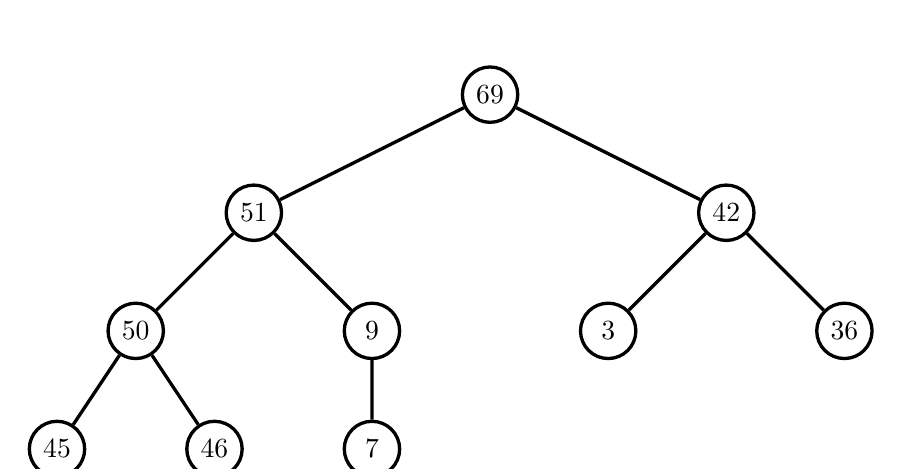
\begin{tikzpicture}[very thick,level/.style={sibling distance=60mm/#1}]
    \node [inheap] {69}
      child {
        node [inheap] {51}
        child {
          node [inheap] {50}
          child {
            node [inheap] {45}}
          child {node [inheap] {46}}
        }
        child {
          node [inheap] {9}
          child {node [inheap] {7}}
        }
      }
      child {
        node [inheap] {42}
        child {
          node [inheap] {3}}
        child {
          node [inheap] {36}}
      };
    \end{tikzpicture}

    \begin{enumerate}
        \item Iteration 1:
        \begin{enumerate}
            \item Swapped \textbf{values}: Compared 51 and 9. Nothing Swapped
        \end{enumerate}
        \item Iteration 2:
        \begin{enumerate}
            \item Swapped \textbf{values}: Compared 46 and (45, 69). Swapped 46 and 69
        \end{enumerate}
        \item Iteration 3:
        \begin{enumerate}
            \item Swapped \textbf{values}: Compared 42 and (3, 36). Swapped 3 and 42
        \end{enumerate}
        \item Iteration 4:
        \begin{enumerate}
            \item Swapped \textbf{values}: Compared 50 and (60, 51). Swapped 50 and 60
        \end{enumerate}
        \item Iteration 5:
        \begin{enumerate}
            \item Swapped \textbf{values}: Compared 7 and (69, 42). Swapped 50 and 60
            \item Swapped \textbf{values}: Compared 7 and (50, 51). Swapped 50 and 60
            \item Swapped \textbf{values}: Compared 7 and 9. Swapped 7 and 9.
        \end{enumerate}
    \end{enumerate}
    % COPY AND PASTE ABOVE TIKZPICTURE AND CHANGE VALUES AS NEEDED
    
    \item Fill in the following images corresponding to the state of the binary tree from (\ref{heap}) at the end of each iteration of the \texttt{for} loop in the \textsc{Heapsort} algorithm. Indicating which values are not considered to be in the heap by setting the node to outheap (from inheap). List which values were swapped in the call to \textsc{Max-Heapify}.

    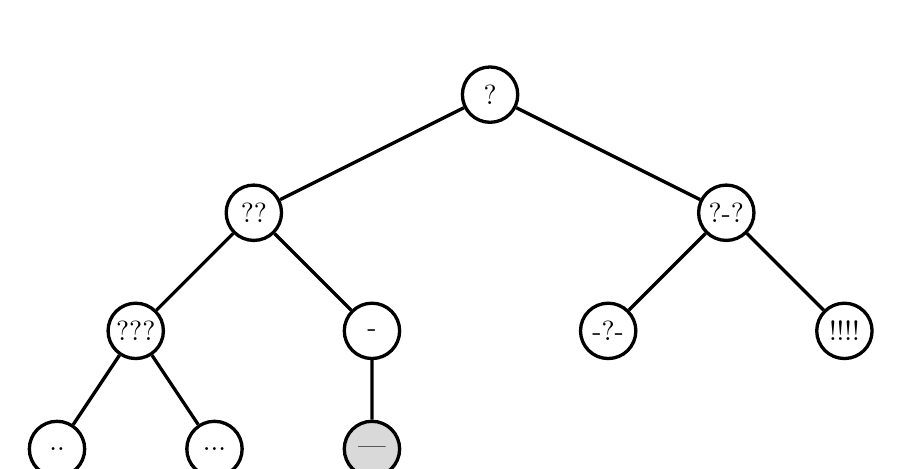
\begin{tikzpicture}[very thick,level/.style={sibling distance=60mm/#1}]
    \node [inheap] {?}
      child {
        node [inheap] {??}
        child {
          node [inheap] {???}
          child {
            node [inheap] {..}}
          child {node [inheap] {...}}
        }
        child {
          node [inheap] {-}
          child {node [outheap] {---}}
        }
      }
      child {
        node [inheap] {?-?}
        child {
          node [inheap] {-?-}}
        child {
          node [inheap] {!!!!}}
      };
    \end{tikzpicture}

    \begin{enumerate}
        \item Iteration 1:
        \begin{enumerate}
            \item Swapped \textbf{values}:
            \item Swapped \textbf{values}:
        \end{enumerate}
        \item Iteration 2:
        \begin{enumerate}
            \item Swapped \textbf{values}:
        \end{enumerate}
    \end{enumerate}

    % COPY AND PASTE ABOVE TIKZPICTURE AND CHANGE VALUES AS NEEDED

    \item Explain (don't prove) why $\lfloor n/2 \rfloor$ calls to \textsc{Max-Heapify} in \textsc{Build-Max-Heap} results in a runtime of $O(n)$ while $n-1$ calls \textsc{Max-Heapify} in \textsc{Heapsort} results in a runtime of $O(n\log n)$.
    
    The build-max-heap runs heapify bottom-up. Most nodes are near the leaves, so their heapify calls are cheap (often O(1) as heapify terminates instantly for leaf nodes). Only a few nodes near the root cost up to O(log n). 
    
    However, for heap sort keep switch the root and the leaf node and uses heapify from the root constantly, which results in O(log n) for all iteration. Since this happens n-1 times, the total cost is O(n log n). 

    % Logical explanation

    \item Analysis of \textsc{Max-Heapify}
    \begin{enumerate}
        \item Write a recurrence equation for \textsc{Max-Heapify} in the worst-case. (Hint: the child of the root of an $n$-node heap is the root of a heap with $\leq \frac{2n}{3}$ nodes)
        
        \begin{center}
            $T(n) = $T($\frac{2n}{3})$ + b (for some positive constant b)\\
        \end{center}

   
        \item Find a tight upper bound for your recurrence and prove that it is correct using induction. 
            \begin{center}
                Level of the tree: $log_\frac{2}{3}n$

                Number of nodes in level i: 1

                Cost per node: 1

                Total Cost in Tree: $log_\frac{2}{3}n$

                Guess: $T(n) = $ O(log n)\\
            \end{center}
            
            Inductive Hypothesis: for all k in [1, n), T(k) $\leq$ c * log(k) for some positive constant c \\
            Inductive Step:\\
            \begin{align*}
                T(n) &\le T\!\left(\Big\lfloor \tfrac{2n}{3} \Big\rfloor\right) + b \\
                &\le c \log\!\left(\tfrac{2n}{3}\right) + b \qquad\\
                &= c\big(\log n + \log \tfrac{2}{3}\big) + b \qquad \text{(} \log(ab)=\log a+\log b \text{)}\\
                &= c\log n + c\log \tfrac{2}{3} + b\\
                &= c\log n - c\log \tfrac{3}{2} + b \\
                &\le c\log n \qquad \text{if } c\log \tfrac{3}{2} \ge b \text{ (e.g., } c \ge \frac{b}{\log(3/2)} \text{)}
            \end{align*}
            
            Let $a > 0$ be the constant runtime when $n\leq 3$. Base Case(s):
            \begin{itemize}
                \item $T(3) = T(2) + b = a + b \leq c \cdot \log 3 + b$ when $a \leq c \cdot \log 3$
            \end{itemize}

            For constants $c = \max\left(\frac{b}{\log(3/2)}, \frac{a}{\log 3}\right)$ and $n \geq 3$, $T(n) \leq c \log n$ holds. Therefore, $T(n) = O(\log n)$.\\
            \end{enumerate}

    \item Analysis of \textsc{Build-Max-Heap}
    \begin{enumerate}
        \item What is the loop invariant of \textsc{Build-Max-Heap}?

        \begin{lemma}[loop invariant]
        ...
        \label{invar}
        \end{lemma}
        
        \item Prove the correctness of \textsc{Build-Max-Heap} using your invariant.

        \begin{proof}
        \textbf{Initialization:} Before the first iteration, $i=?$.  In this case, the loop invariant says ... This is true because ...
        
        \textbf{Maintenance:} Assume that the loop invariant is true before some iteration $i$, that is, ... During iteration $i$, ... Before the next iteration of the loop, $i$ is ...  Once this happens, our conclusion is rewritten as ``...''  Therefore, the maintenance step holds.
        \end{proof}
        
        \begin{lemma}[loop termination condition]
        After the for loop terminates, ...
        \label{term}
        \end{lemma}
        
        \begin{proof}
        In the final iteration of the outer for loop, $i = ?$. Therefore, ...
        \end{proof}
        
        \begin{theorem}
        \textsc{Build-Max-Heap} correctly ...
        \end{theorem}
        
        \begin{proof}
        According to Lemma \ref{term}, after the loop, ... Therefore, we can conclude that \textsc{Build-Max-Heap} correctly ...
        \end{proof}
    \end{enumerate}
    
\end{enumerate}
\end{document}